%
% GNU courseware, XIN YUAN, 2018
%

\section{进程和线程}

\frame{
\centerline{\textbf{\Huge{进程和线程}}}
}

\frame{\frametitle{代码的目标形式}
桌面程序仍然是科研和工程中软件的主要形式,主要类型有:

\begin{table}[htbp]
\centering
\begin{tabular}{|p{0.4\textwidth}|p{0.4\textwidth}|}
\hline
\textcolor[rgb]{0.0, 0.0, 1.0}{Windows} & \textcolor[rgb]{0.0, 0.0, 1.0}{Linux} \\
\hline
界面程序(UI)         & 一般进程调用界面库 \\
\hline
控制台程序(Console)  & 一般进程 \\
\hline
服务程序(Service)    & 守护进程 \\
\hline
\end{tabular}
\end{table}
}

\frame{\frametitle{代码的目标形式}
运行在平台上的程序还有一类是\textbf{脚本程序},是以一个特定的桌面程序作为宿主平台,
读取文本或者二进制形式的脚本程序,解释执行。主要有:
\begin{enumerate}
\item<1-> web应用程序(服务器端脚本,客户端在浏览器中运行的各种脚本程序)
\item<2-> 办公软件(word, excel之VBA,SQLServer中存储过程等)
\item<3-> 科学计算程序(matlab, mathematic, mathCAD, AutoCAD, 3DMax, Photoshop, Python等)
\item<4-> 游戏动画(3D游戏引擎下的如lua等脚本)
\end{enumerate}
}

\frame{\frametitle{什么是进程?}
\begin{enumerate}
\item<1-> Windows任务管理器,Linux下ps –e命令。
\item<2-> \textbf{进程}(Process)是操作系统多任务并发执行的一个基本单位。
\item<3-> 一个可执行文件(exe或x)可以启动多个进程\textbf{实例}。展示。
\item<4-> 在程序里编写特殊代码可以使其只能启动一个进程。
\end{enumerate}
}

\frame{\frametitle{什么是线程?}
\begin{enumerate}
\item<1-> Windows任务管理器,Linux下ps –eLF命令。
\item<2-> 在进程中可以利用程序代码来动态地创建\textbf{线程}(Thread),
作为多任务并发执行的补充。进程可创建一个或多个线程,
每个线程都独立地同时执行一段相同或不同的程序。
\item<3-> Windows中启动一个进程的同时也创建了一个\textbf{主线程},
这个线程和该进程同时存在,不能被程序代码动态消灭,只有进程被终止时才会消失。
\item<4-> Linux的线程是用库实现的轻量级进程。
\end{enumerate}
}

\frame{\frametitle{直观理解}
线程内的代码是一个逻辑上完整的任务。但是在执行时可以被操作系统打断,
在各个时间片内获得CPU、缓存、内存、硬盘永久存储(或者其他外设,如GPU)
等资源来执行其中的一小段代码。
}

\frame{\frametitle{进程空间}
进程与内存:
\begin{enumerate}
\item<1-> 进程与进程之间能访问的内存空间是相互隔离的。
\item<2-> 每个进程拥有自己独立编址的内存空间(称为虚拟内存空间),
在32位操作系统下最大达4G,在64位操作系统下更大。 
\item<3-> 操作系统把进程的虚拟内存空间按多个固定大小的内存页面来组织,
分为可交换页和非可交换页两种。非可交换页常驻物理内存,
可交换页由操作系统根据程序运行的需要调入物理内存来访问或者执行代码,
在不需要时换出物理内存,存储到硬盘上。
\item<4-> 内存页的内容就是可执行的程序代码以及相关的数据。
\end{enumerate}
}

\frame{\frametitle{进程空间}
线程与内存:

~

线程是由进程的程序创建的,因此它们属于创建它们的进程,
进程的内存空间对它们来说都是透明的,即每个线程都可以访问该进程的内存空间。
显然,当多个线程读/写相同的内存数据时,就会发生冲突。
操作系统提供解决冲突的编程方法。
}

\frame{\frametitle{进程调度}
现代计算机的CPU一般有多个核,主流是2-16核,将来还有更多。
从Windows任务管理器看到通常有近百进程,上千线程在执行,
所以实际上这些进程和线程不可能同时在有限的核上并发执行。
操作系统需要对这些进程或者线程进行调度,使得每个线程都能轮流执行一个小的时间段,
从而使CPU利用率最大。Windows以线程为多任务并发基本调度单位,
Linux则以进程为多任务并发基本调度单位。
}

\frame{\frametitle{进程调度}
\begin{itemize}
\item<1-> Windows下一个进程可创建1000线程,不会引起效率的显著下降。
\item<2-> Linux下一个进程可创建300线程,不会引起效率的显著下降。
\end{itemize}
}

\frame{\frametitle{进程与装配件}
\begin{enumerate}
\item<1-> 操作系统以可执行文件为“蓝图”来创建一个进程。
\item<2-> 可执行文件包含有代码和数据,称为一个程序集。
\item<3-> 操作系统根据可执行文件的内容,为进程分配内存页,
把可执行文件的代码和数据映射到这些内存页上。
\item<4-> 如果同一个可执行文件启动了两个或更多的进程,
则有部分相同的代码或数据内存页面可以在多个进程间共享,
从而减少了整机的内存消耗。
\end{enumerate}
}

\frame{\frametitle{进程与装配件}
\begin{itemize}
\item<1-> 可执行文件加载到进程后,操作系统会根据文件信息找到它的入口地址,
从该地址执行机器码(也就是该进程或主线程在执行这些代码)。
\item<2-> 可执行文件可以用来装配一个进程的内容,
所以又被称为装配模块(module)或者装配件(Assembly)。
\item<3-> 还有两种类型的装配件,一是共享库(DLL或SO),二是驱动程序(driver)。
\end{itemize}
}

\frame{\frametitle{装配件}
\begin{table}[htbp]
\centering
\begin{tabular}{|p{0.4\textwidth}|p{0.4\textwidth}|}
\hline
\textcolor[rgb]{0.0, 0.0, 1.0}{Windows} & \textcolor[rgb]{0.0, 0.0, 1.0}{Linux} \\
\hline
可执行模块exe(自身代码引用的地址全部已确定) & 可执行模块(同左) \\
\hline
动态链接模块DLL(自身代码引用地址为浮动地址,必要时需要重定位)  & 共享库模块SO.X(同左) \\
\hline
驱动程序模块SYS或其他,运行在核心态/用户态  & 驱动程序模块,运行在核心态/用户态 \\
\hline
\end{tabular}
\end{table}
}

\frame{\frametitle{装配件}
\begin{itemize}
\item<1-> 共享库的代码和数据,相同的部分可以在进程间共享。
\item<2-> 共享库通过导出函数供其它装配件来使用。
\item<3-> VS的DLL工程输出目标是DLL文件(带.dll后缀名),
同时还生成\textbf{导入库}(.lib后缀的文件)。
导入库包含该DLL的导出函数的列表,不含真实的代码。
\item<4-> g++生成SO文件,不产生导入库。
\end{itemize}
}

\frame{\frametitle{装配件}
\begin{itemize}
\item<1-> 可执行文件记录它需要使用的共享库文件名及引出函数名。
此时可执行文件在生成时需要和DLL配套的\textbf{导入库}链接(隐式链接),
或直接在 SO文件中查找。
\item<2-> 程序中也有可以由代码(API函数调用)动态加载DLL/SO,
并取得它导出的函数地址,再调用(显式链接)。
\item<3-> 一个DLL/SO可以被多个可执行文件使用,从而整体上节约了内存页的使用。
\end{itemize}
}

\frame{\frametitle{装配件}
\begin{itemize}
\item<1-> 当一个可执行文件被加载到一个进程中时,操作系统会根据该文件中共享库信息,
把需要的共享库加载到内存页面中,并映射到该进程。如果该共享库在其它进程中已经被加载,
那么操作系统不会重复加载,直接把相同的代码和数据页面映射到本进程,
只为不同的部分分配本进程使用的新的内存页面。动态加载共享库与此类似。
\item<2-> 所以把可能被多个可执行程序使用的公共函数放到共享库中能加快运行速度,
节约内存的使用。
\end{itemize}
}

\frame{\frametitle{装配件}
\begin{itemize}
\item<1-> DLL/SO文件内程序引用的全局数据地址、记录的导出函数地址都是浮动地址,
在加载(装配)过程中被重新定位,从而使得进程中来自其他装配件的程序代码能够访问和调用它们。
\item<2-> DLL/SO文件同样会记录它需要使用到的其他DLL/SO的文件名及DLL/SO中的函数名。
在进程装配时,如果该DLL/SO装配件依赖其它DLL/SO装配件,则操作系统会递归地依次装入它们。
\end{itemize}
}

\frame{\frametitle{装配件}
\begin{itemize}
\item<1-> 驱动程序,也是一种装配件模块,其代码和数据被映射到进程的特殊内存地址区域,
如win32下它们被映射到2G以上的内存地址。
\item<2-> 驱动程序代码提供的服务程序,在CPU的核心态(ring0级别)运行,
是受操作系统信任的程序。
\item<3-> 驱动程序的内存页面分为可分页(paged)和非分页(non-paged)两种,
后面的内存页面常驻物理内存,前面的页面可以和磁盘文件交换。
\end{itemize}
}

\frame{\frametitle{装配件}
驱动程序的代码和数据在开机时就被操作系统分配内存页面并装入,
在每个进程启动时,会把它们映射到进程的特殊地址上,
因此驱动程序的内存页面是系统中所有进程共享的。
}

\frame{\frametitle{装配件}
一个进程由一个可执行装配件(含主入口程序)、一个或多个共享装配件
(某些可执行装配件被动态装载时,算作动态装配件)、驱动程序装配件组成。
}

\frame{\frametitle{示意图}
\noindent
\begin{figure}[h]
\centering
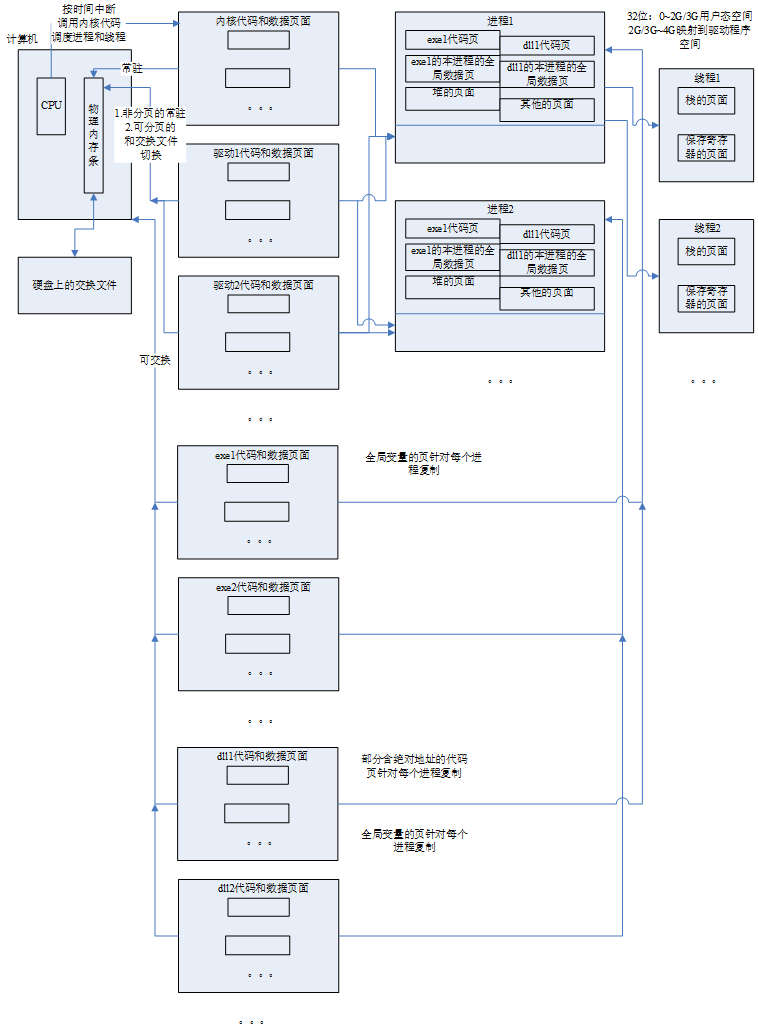
\includegraphics[width=0.5\textwidth]{topics/process-files/show.png}
\end{figure}
}

\frame{\frametitle{装配件的组成}
\begin{itemize}
\item<1-> 机器代码
\item<2-> 已初始化全局数据(如\textbf{全局变量}、\textbf{静态成员变量})
\item<3-> 未初始化全局数据(如方法/函数内的\textbf{静态局部变量})
\item<4-> 资源(在Windows下的exe或DLL内,可看作特殊的全局数据)
\item<5-> 模块信息(各种信息及导入/导出函数表)
\end{itemize}
}

\frame{\frametitle{装配件的组成}
\begin{itemize}
\item<1-> 装配件(可执行和共享)中的机器代码可以在不同的进程间共享(因为大部分内容都相同)。
\item<2-> 资源是只读的,可以在不同的进程间共享。
\item<3-> 全局性数据一般不能共享,操作系统会为每个使用此装配件的进程建立专属于该进程的私有内存页,
存放全局数据,即每个进程都复制了一份全局数据的独立拷贝。
\end{itemize}
}

\frame{\frametitle{装配件的组成}
\begin{itemize}
\item<1-> 可以在代码中编写特殊的设置,当生成装配件时让全局性数据可以在不同的进程间共享,
但一般不推荐这样作,而是用\textbf{共享内存}技术来取代。
\item<2-> 模块信息大部分都是只读信息,因此在不同进程中的内容都相同,可以在进程间共享。
\end{itemize}
}

\frame{\frametitle{装配件的组成}
模块信息中和导入函数表相关的有一段stub代码,是一些跳转指令,
跳转到导入函数的调用地址,这样本装配件模块的程序就能调用导入函数了。
因为导入函数所在的共享库在不同的进程中可能会被装入相同的地址,
此时stub里的跳转地址都是相同的,可以在进程间共享;
也可能被装入不同的地址,操作系统为其分配进程私有内存页来存放。
}

\frame{\frametitle{装配件的组成}
\begin{itemize}
\item<1-> 所以共享库是一种\textbf{二进制级别}的代码复用方法。
\item<2-> C++程序(类、函数等)则是\textbf{源代码级别}的代码复用方法。
因为源代码若修改了整个软件都要重新编译。
\item<3-> 编写大型工程/算法软件时一般都需要进行装配件模块的分划和设计。
\end{itemize}
}

\frame{\frametitle{全局变量的问题}
\begin{itemize}
\item<1-> 程序中的全局变量、类的静态成员变量、方法/函数内的静态局部变量
(线程局部存储变量除外)都是全局性的数据,如果源代码中存在有这样的变量,
会在生成的装配件里有自己唯一的一个虚拟内存地址
(可执行文件中是确定的地址,共享库中是浮动地址)。
\item<2-> 如果一个解决方案里含可执行工程及其依赖的多个共享库工程,
每个工程中都使用了上面的源代码,那么可执行文件执行时的进程内将会有多份这样的全局性数据
(分别位于可执行文件和多个共享库的内存页面中)。
\end{itemize}
}

\frame{\frametitle{全局变量的问题}
如果算法设计中需要的一个全局性变量是相对整个进程来说是唯一的,
就不能把含有该全局性变量的代码做成源代码级别的共享库
(共享库可能会被多个工程使用,从而产生多份全局数据),
而是做在一个单独的共享库内,再通过一系列导出函数来操作该变量。
}

\frame{\frametitle{多线程的问题}
\begin{minipage}[t]{0.9\textwidth}
\noindent
\textbf{多线程}:一个进程可以创建多个线程,而这些线程是可以并行访问同一进程空间内的数据的,
因此要注意对可能会被多个线程访问和修改的数据进行\textbf{同步保护}。

~

\noindent
\textbf{例子}:
\end{minipage}

~

\begin{minipage}[b]{\textwidth}
\noindent
\begin{figure}[hb]
\centering
\uncover<2->{
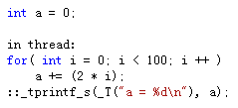
\includegraphics[width=0.4\textwidth]{topics/process-files/mt1.png}
}
~
\uncover<3->{
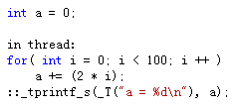
\includegraphics[width=0.4\textwidth]{topics/process-files/mt2.png}
}
\end{figure}
\end{minipage}
}

\frame{\frametitle{多线程的问题}
整个过程若不保护,当两个线程都执行上面的代码时,因数据被修改的先后顺序不可预测,
所以最终打印的结果不是预先设想的结果,即不可预测。不同线程的输出结果会不同,
在不同机器上跑的结果也可能都不同。
}

\frame{\frametitle{多线程的问题}
全局性的变量要特别注意进行多线程保护,特别是方法/函数内的静态局部变量,
它是在第一次被调用时才被初始化的,如果有多个线程同时调用该方法/函数而不注意保护,
可能会造成该静态局部变量被多次初始化
(含静态局部变量的方法/函数被称为\textbf{不可重入}的)。
}

\frame{\frametitle{同步对象}
操作系统提供了一些内核对象,既可以在多线程环境下保护(同步)进程中数据的读写,
也可以在多进程环境下保护(同步)能在进程间共享的内核对象的操作。
}

\frame{\frametitle{Windows下同步对象}
\begin{table}[htbp]
\centering
\begin{tabular}{|p{0.2\textwidth}|p{0.4\textwidth}|p{0.3\textwidth}|}
\hline
\textcolor[rgb]{0.0, 0.0, 1.0}{同步对象} & \textcolor[rgb]{0.0, 0.0, 1.0}{线程} & \textcolor[rgb]{0.0, 0.0, 1.0}{进程} \\
\hline
互斥量   & 关键段CriticalSection和匿名Mutex       & 命名Mutex \\
\hline
信号量   & 匿名Semaphore & 命名Semaphore \\
\hline
条件变量 & CONDITION\_VARIABLE变量配合关键段或读写锁 & 无 \\
\hline
读写锁   & SRWLOCK变量   & 无 \\
\hline
事件触发 & 匿名Event     & 命名Event \\
\hline
\end{tabular}
\end{table}
}

\frame{\frametitle{Linux下同步对象}
\begin{table}[htbp]
\centering
\begin{tabular}{|p{0.2\textwidth}|p{0.5\textwidth}|p{0.2\textwidth}|}
\hline
\textcolor[rgb]{0.0, 0.0, 1.0}{同步对象} & \textcolor[rgb]{0.0, 0.0, 1.0}{线程} & \textcolor[rgb]{0.0, 0.0, 1.0}{进程} \\
\hline
互斥量   & mutex  & mutex \\
\hline
信号量   & sem    & sem \\
\hline
条件变量 & condition变量配合mutex & 无 \\
\hline
读写锁   & rwlock & rwlock \\
\hline
\end{tabular}
\end{table}
}

\frame{\frametitle{同步的效果}
从程序的执行过程分析,通过内核对象的同步保护后,数据的访问在时间顺序上变成了串行的,
即不再有多个线程同时读/写数据,而是按顺序依次读/写它们,从而不会再有访问冲突,
也不会出现不可预测的结果。
}

\frame{\frametitle{装配件内存问题}
\begin{itemize}
\item<1-> CRT库中隐含有全局变量。采用动态链接方式没有问题,
但若采用静态链接方式将使每个装配件模块都有一份这样的全局变量。
如new,malloc等动态内存分配函数会使用隐含的全局变量来标识内存分配的内部数据结构。
\item<2-> 静态链接方式下,在一个模块中的函数分配内存,
在另一个模块中的函数释放这块内存,会导致内存错误。
这是因为它们各自使用了不同的全局变量来操作内存分配。
而上述分配的内存指针只能由第一个模块来有效处理,
用第二个模块来释放时,就会出现不可预测的错误。
\item<3-> 所以编写代码时要在同一个模块内同时提供内存的分配和释放的函数。
\end{itemize}
}

\frame{\frametitle{全局对象的构造}
全局变量的构造方法调用之间不能有\textbf{依赖}关系。
编译器会在程序入口处为全局变量的初始化生成代码。
有些全局变量是用常量初始化的,已经记录在全局数据内存区,不需要再初始化;
有些全局变量需要调用构造方法,它们的调用顺序则是不确定的。
如果构造方法之间有依赖关系,会出现不可预知的错误。
}

\frame{\frametitle{其他}
\begin{itemize}
\item<1-> 所以进行算法设计时尽量少用全局变量,包括少用线程局部存储TLS全局变量。
\item<2-> TLS全局变量在每个线程中都会有一份该变量的拷贝,各自独立操作。
如CRT库中数学函数调用会设置一个错误变量errno,用来标明数学函数调用是否发生了错误。
DOS单线程编程时代被定义成全局变量,多线程编程下显然数学函数可能会被多个线程同时调用,
该变量的设置就会发生冲突,从而根据该变量判断是否有错变得不可预测。
现在的CRT将其设置为TLS就使得该变量是线程安全的。
\end{itemize}
}

\frame{\frametitle{其他}
\begin{itemize}
\item<1-> 尽量使用类的成员变量来描述问题中的属性、状态等。
\item<2-> 即使必须要使用全局性的变量,也要控制在一定范围内,
要考虑进程范围、线程范围、模块范围的内存占用情况和使用情况,
构造方法不能相互依赖,要不要\textbf{同步保护}等。
\end{itemize}
}

\frame{\frametitle{参考书}
{\CJKfamily{zhkai}
\begin{itemize}
\item<1-> 《Linker and Loader》
\item<2-> 《设计模式》
\end{itemize}
}
}

%end
